\documentclass[12pt,a4paper]{article}

% --------------------
% Packages
% --------------------
\usepackage[utf8]{inputenc}
\usepackage[T1]{fontenc}
\usepackage{lmodern}
\usepackage{amsmath}
\usepackage{amssymb}
\usepackage{graphicx}
\usepackage{booktabs}
\usepackage{subcaption}

\usepackage{natbib}
\usepackage{xurl}
\usepackage[hidelinks]{hyperref}

% Approx. 3 cm margins as required by Trier
\usepackage[
    a4paper,
    left=3cm,
    right=3cm,
    top=3cm,
    bottom=3cm
]{geometry}

% 1.5 line spacing
\usepackage{setspace}
\onehalfspacing

% Better typography
\usepackage{microtype}

% Prevent headings being stranded at bottom of page
\usepackage{needspace}

% --------------------
% Widow / orphan control
% --------------------
\widowpenalty=10000
\clubpenalty=10000
\displaywidowpenalty=10000

\begin{document}
\pagenumbering{gobble}
% ==================================================
% TITLE PAGE
% ==================================================

\begin{titlepage}
    \thispagestyle{empty}

    \begin{center}

        % University
        {\Large\textbf{Universität Trier}\par}

        \vspace{0.3cm}

        {\large Department of Computerlinguistik and Digital Humanities\par}

        \vspace{0.15cm}

        \vspace{1.8cm}

        % Document type
        {\large\textbf{Term Paper}\par}

        \vspace{0.5cm}

        {\large
        Advanced Topics in Computational Text and Media Sciences 1
        \par}

        \vspace{0.25cm}

        {\normalsize Summer Semester 2026\par}

        \vspace{2cm}

        % Title
        {\LARGE\bfseries
        Does BERT Really Know Grammar?
        \par}

        \vspace{0.4cm}

        {\Large\bfseries
        Stress-Testing Attention Probes with Control Tasks
        \par}

        \vfill

        % Author information
        \begin{tabular}{@{}rl@{}}
            \textbf{Lecturer:}
            & Kai Kugler, M.A. \\[0.35cm]

            \textbf{Author:}
            & Swathi Raya \\[0.35cm]

            \textbf{Degree Programme:}
            & M.Sc. Natural Language Processing \\[0.35cm]

            \textbf{Semester:}
            & 1st Semester \\[0.35cm]

            \textbf{Matriculation Number:}
            & 1776241 \\[0.35cm]

            \textbf{E-mail:}
            & rayaswathi2601@gmail.com
        \end{tabular}

        \vfill

        % Submission
        {\large
        \textbf{Submission Date}
        \par}

        \vspace{0.15cm}

        {\large 28 September 2026\par}

    \end{center}
\end{titlepage}

% ==================================================
% ABSTRACT
% ==================================================

\section*{Abstract}

% We will write the abstract here later.
Large pretrained language models such as BERT have demonstrated that they are able to encode significant amounts of linguistic information, but does high probing accuracy really reflect the fact that this information is actually represented in the model? An expressive enough probe can learn to recognize patterns in the data that have nothing to do with the representation that it is trying to understand. This paper explores the question of how accurately can syntactic information be recovered from BERT attentions by looking at the relationship between probing accuracy and the performance of the same probe trained on an unrelated control task.

Using attention features extracted from BERT-base-uncased on the dependency relations from the Universal Dependencies English Web Treebank, we investigate two probing tasks -- predicting the presence of a dependency relation and predicting its type. To separate linguistic signals from probe memorization effects, we look at selectivity, the difference in performance between the real task and a control task with arbitrary labels. We conduct three sets of experiments: investigating the selectivity of various baseline probes, examining how increasing the representational capacity of the probe impacts selectivity and accuracy, and analyzing the distribution of syntactic information across different layers of BERT. We find that there is not always a correlation between raw probing accuracy and selectivity. By increasing the capacity of the probe we were able to improve task accuracy while also increasing the accuracy on control labels, thus lowering the selectivity. We also find that syntactic information is present in many of BERT's attention layers, with layer 7 showing the most promise for both task types, as evidenced by the selectivity scores. Our experiments demonstrate that control tasks should be used when analyzing probing results.

\newpage

% ==================================================
% TABLE OF CONTENTS
% ==================================================

\thispagestyle{empty}
\tableofcontents
\newpage

% ==================================================
% MAIN PAPER
% ==================================================
\pagenumbering{arabic}
\setcounter{page}{1}

\section{Introduction}

Pre-trained Transformer language models have revolutionized Natural Language Processing by learning contextual representations of language from enormous bodies of text. Bidirectional Encoder Representations from Transformers (BERT) is one such model, and has motivated a flurry of follow-up research investigating the sorts of linguistic information that are reflected in its representations \cite{devlin2019bert}. Of interest to this work is whether BERT reflects syntactic structure, despite not being trained as a dependency parser.

Various works have suggested that BERT does contain grammatical information, either in its self-attention patterns \cite{clark2019what}, or in the representations of its intermediate layers \cite{tenney2019bert}. However, these claims typically rest on syntactic \emph{probing}: training a classifier to recognize a syntactic phenomenon in a BERT representation. While high accuracy on such a probe suggests that some information is encoded in the representation, it is not always clear that the information is \emph{clearly} encoded, as an expressive probe may memorize patterns specific to the task.

Hewitt and Liang tackle this issue using \emph{control tasks}: variant classification tasks in which the true linguistic label is replaced by an arbitrary assignment, while retaining potential for the probe to memorize patterns in the control labels \cite{hewitt2019designing}. The degree to which a probe generalizes from the linguistic to the control task is termed its \emph{selectivity}: ideally, a good probe should perform well on the linguistic task, and poorly on controls.

This paper investigates the extent to which such control-task selectivity supports the claim that syntactic dependency information can be recovered from BERT attention, and how this support varies with probe capacity and BERT layer. Attention weights from \texttt{bert-base-uncased} are probed on two linguistic tasks: whether a dependency relation exists between two words, and what that relation is. The three main experiments are as follows:

\begin{quote}

\textit{What is baseline performance on the linguistic and control tasks, for varying probe capacities? To what extent does increasing probe capacity increase selectivity? How does selectivity vary with BERT layer?}

\end{quote}

The work is restricted to \texttt{bert-base-uncased}, English dependency syntax, attention-weight representations, and a limited set of probe architectures. As such, the findings are not necessarily generalizable to other languages, models, or representation types; a comparison with a randomly-initialized BERT is left to future work.

Section~2 covers related work on BERT attention, syntactic representations, probing, and selectivity. Section~3 describes the methodology, Section~4 gives the experimental results, Section~5 discusses their implications and limitations, and Section~6 concludes and suggests future work.

% ==================================================
% 2. BACKGROUND AND RELATED WORK
% ==================================================

\section{Background and Related Work}

\subsection{BERT and self-attention}

BERT is a Transformer-based language model that learns bidirectional contextual representations from unlabeled text \cite{devlin2019bert}. In contrast to earlier approaches where word representations were largely independent from context, BERT represents each token according to the sentence that it is in. This is achieved by stacked Transformer layers that perform self-attention and thus allow each token to assign different weights to different other tokens.

BERT uses multi-head self-attention where several attention heads perform in parallel. Each head provides a matrix that describes the strength of attention from one token to another. While these patterns are not explicitly learned with reference to syntactic phenomena, they have provided motivation for investigating whether certain heads or layers of BERT contain recognizable linguistic information.

In general, it has been found that BERT representations encode various types of linguistic information. Rogers et al.\ stress, however, that showing that information can be recovered from a representation is different from showing that the model uses that information for prediction \cite{rogers2020primer}. This is a particularly relevant caveat in the case of attention patterns as linguistic representations.

\subsection{Syntactic information in BERT}

Several works have investigated whether BERT encodes syntactic information. Clark et al.\ show that some attention heads correspond strongly to specific linguistic relations, including determiners attending to nouns and verbs attending to direct objects \cite{clark2019what}. These results imply that combinations of BERT attention heads can provide substantial syntactic information.

Layer-wise analyses suggest that this information does not appear uniformly across the network. Tenney et al.\ find a progression across BERT layers akin to a traditional NLP pipeline, with syntactic information becoming particularly prominent in intermediate parts of the network \cite{tenney2019bert}. This has motivated the investigation of individual layers rather than considering the full network as a whole.

The intuition of a layer-wise linguistic pipeline, however, is not undisputed. Niu et al.\ argue that the relationship between linguistic function and BERT layer depth is not conclusively established and that other factors may play a role \cite{niu2022pipeline}. The present study therefore analyzes each layer individually with the same probing and control-task procedure rather than making prior assumptions about where syntactic information might be found.

\subsection{Probing classifiers}

Probing classifiers are a tool for investigating what information can be recovered from neural representations. A probe is trained to predict some linguistic property while the underlying language model is held fixed. Probing results are often reported as evidence that the model has encoded the relevant kind of information, if a probe is able to predict linguistic properties successfully.

An important caveat to this approach is that the performance of a probe depends on two factors: the representation and the classifier itself. A complex classifier could learn to make use of decision boundaries that are not relevant to the linguistic phenomenon of interest or even memorize associations specific to the probing data. As a result, higher accuracy for a probe is not necessarily indicative of better linguistic encoding. This distinction between information contained in the representation and information learned by the probe is a key consideration in probing methodology, according to Belinkov \cite{belinkov2022probing}.

The capacity of a probe therefore matters. A linear classifier has limited representational power, while a multilayer perceptron can learn more complicated decision boundaries. If both linguistic-task and arbitrary-task performance increase as probe capacity increases, then raw accuracy is not a particularly informative measure. This consideration motivates the probe-capacity experiment in the present study.

\subsection{Control tasks and selectivity}

Hewitt and Liang suggest using control tasks to measure the extent to which a probe has learned arbitrary associations with the labels of interest \cite{hewitt2019designing}. A control task is similar to the original linguistic task, but with arbitrary labels in place of linguistic ones. Performance on the control task therefore indicates how much the probe has been able to memorize about the association between representations and label assignments.

They define \emph{selectivity} as the difference between real-task accuracy and control-task accuracy:

\begin{equation}
\text{Selectivity}
=
\text{Accuracy}_{\text{real}}
-
\text{Accuracy}_{\text{control}}.
\end{equation}

A probe is more selective if it achieves high accuracy for the linguistic task while performing comparatively poorly on the control task. The most accurate probe therefore does not necessarily provide the most insight into the representation.

Follow-up works have investigated this idea further, providing additional criteria for evaluating probing results. Information-theoretic approaches, for example, offer an alternate perspective on the evaluation of probes and establish links between information-based measures and selectivity \cite{zhu2020information}. In general, these works highlight the need to interpret raw classification accuracy with care.

The present study adopts the general approach of Hewitt and Liang and applies it to syntactic information recoverable from BERT attention. It investigates three interconnected questions: whether dependency information can be predicted from attention, how this interpretation changes with probe capacity, and whether selectivity differs across BERT layers.


% ==================================================

% 3. METHODOLOGY

% ==================================================

\section{Methodology}

\subsection{Study Design}

This study uses a controlled probing framework to examine whether syntactic dependency information can be recovered from BERT self-attention and how this interpretation changes with probe capacity and model depth. BERT remains fixed throughout the experiments: attention values are extracted once, stored as feature vectors, and then used to train separate classifiers on linguistic and control tasks. This ensures that the experiments evaluate information already present in the pretrained representations rather than information introduced through task-specific fine-tuning.

Two probing tasks are considered. The \emph{dependency-existence} task predicts whether two words are connected by a dependency relation, while the \emph{dependency-type} task predicts the grammatical relation between a dependent and its syntactic head. Three experiments are conducted: a baseline selectivity experiment using the full attention representation, a probe-capacity experiment comparing classifiers of different complexity, and a layer-wise experiment examining individual BERT layers.

\subsection{Dataset and Pair Construction}

The experiments use version r2.18 of the Universal Dependencies English Web Treebank (UD English EWT) \cite{silveira2014gold}. The corpus provides English sentences annotated with dependency heads and relation labels. Training, development, and test files are processed separately, and multiword-token ranges are removed during preprocessing.

For each sentence, every dependency except the root relation is converted into an ordered dependent--head pair. The dependency label is retained for the dependency-type task. For dependency existence, these annotated pairs form the positive examples. Negative examples are sampled from within-sentence word pairs that are not dependency relations. Self-pairs and genuine dependencies in either direction are excluded, and approximately one negative example is sampled for each positive example. Negative sampling starts from seed 13 and varies reproducibly by sentence. Although pair files are created for all three corpus splits, the reported probes are trained on the training split and evaluated on the test split. The development split is not used for model selection.

\subsection{Attention Feature Extraction}

Each word pair is represented using attention weights from \texttt{bert-base-uncased}. A fixed model revision is used, the model is run in evaluation mode, and no fine-tuning is performed. Because BERT operates on WordPiece tokens, the original treebank words are aligned with their corresponding subword indices. If either word is split into multiple WordPieces, attention values across all relevant subword combinations are averaged separately for each attention head.
BERT-base contains 12 Transformer layers with 12 attention heads per layer. Each word pair is therefore represented by a 144-dimensional vector,

\begin{equation}
\mathbf{x}_{ij} \in \mathbb{R}^{144}.
\end{equation}

Each dimension represents the mean attention value for one layer--head combination. For genuine dependencies, the direction is from the dependent to its syntactic head. The resulting vectors are cached before probe training so that linguistic and control tasks use exactly the same input representations. If a word is unavailable after BERT truncation, the corresponding pair is skipped. BERT is run once per sentence, after which features are extracted for all pairs in that sentence.

\subsection{Probing Tasks}

The dependency-existence task is a binary classification problem. Positive examples are annotated dependency pairs, while sampled non-dependency pairs form the negative class. The probe receives the 144-dimensional attention vector and predicts whether a dependency relation exists between the two words.

The dependency-type task is evaluated only on genuine dependency pairs. Relation labels are ranked by frequency in the training data; the 20 most frequent labels are retained individually and all remaining relations are mapped to a shared \texttt{other} class. The resulting label set is fixed from the training data and reused for evaluation. These tasks examine two levels of syntactic information: whether a dependency exists and, when it does, what grammatical relation it expresses.

\subsection{Control Tasks and Selectivity}

Control tasks are used to estimate how much performance can be obtained from arbitrary word--label associations rather than from meaningful syntactic structure. The BERT attention features remain unchanged; only the target labels differ.

For dependency existence, each lowercased training-vocabulary word type is randomly assigned to one of two arbitrary classes. A pair receives a positive control label when both words belong to the same class and a negative label otherwise. The control vocabulary is generated with seed 42 and applied consistently to both training and test data.

For dependency type, each word type is assigned an arbitrary dependency label. Labels are sampled according to the empirical distribution of the real training labels rather than uniformly, preserving the approximate class-frequency structure of the original task. The dependent word determines the control label for each pair.

Selectivity is defined as

\begin{equation}
S = A_{\mathrm{real}} - A_{\mathrm{control}},
\end{equation}

where \(A_{\mathrm{real}}\) is accuracy on the linguistic task and \(A_{\mathrm{control}}\) is accuracy on the corresponding control task. A larger value indicates stronger separation between meaningful linguistic prediction and arbitrary-label learning.

\subsection{Probe Architectures and Evaluation}

The baseline classifier is logistic regression trained directly on the attention vectors. In the probe-capacity experiment, it is compared with multilayer perceptrons containing one hidden layer of 8 and 32 units. Logistic regression uses a maximum of 1000 optimization iterations, while both MLPs use a maximum of 500. The goal is not to optimize the strongest possible classifier, but to observe how linguistic accuracy, control accuracy, and selectivity change as probe capacity increases.

Experiments are run with five configured seeds: 13, 42, 97, 1000, and 2024. Mean accuracy and standard deviation are recorded for the real and control tasks, and selectivity is calculated from the difference between the corresponding mean accuracies. Before the capacity and layer-wise analyses, the cached feature matrices used by the real and control experiments are checked for equality.

For the layer-wise experiment, the full 144-dimensional representation is divided into 12 groups of 12 dimensions, one group for each BERT layer. A linear probe is trained on each layer separately. A dimensionality-matched baseline is also created by sampling 12 attention dimensions without replacement from the full representation using seed 42. This comparison tests whether coherent attention heads from the same layer provide more syntactic information than an arbitrary 12-dimensional subset.

% ==================================================
% 4. EXPERIMENTS AND RESULTS
% ==================================================

\section{Experiments and Results}

This section presents the results of the three experiments. The first establishes a baseline using the complete 144-dimensional BERT attention representation and a linear probe. The second examines whether increasing probe capacity changes the relationship between linguistic-task accuracy and control-task performance. The third evaluates individual BERT layers to determine whether selectivity is distributed uniformly across the model or concentrated at particular depths. Because the central aim of the study is to distinguish raw predictive performance from evidence of linguistic encoding, both accuracy and selectivity are considered throughout.

\subsection{Experiment 1: Baseline Selectivity}

The first experiment uses a linear probe over the complete 144-dimensional attention representation. For the dependency-existence task, the probe achieves a real-task accuracy of 0.8404 and a control-task accuracy of 0.5065, corresponding to a selectivity of 0.3339. For dependency-type prediction, real-task accuracy is 0.7130 and control-task accuracy is 0.3116, producing a higher selectivity of 0.4014.

These results establish a substantial separation between performance on the genuine linguistic tasks and the corresponding arbitrary control tasks. In both cases, the probe performs considerably better when the target labels represent actual syntactic information. The baseline therefore provides evidence that BERT attention contains recoverable information about both the existence and type of dependency relations. At the same time, the non-trivial control accuracies show why raw task accuracy alone is insufficient for interpreting the probe.

\subsection{Experiment 2: Effect of Probe Capacity}

The second experiment investigates whether increasing the expressive capacity of the probe strengthens or weakens this interpretation. A linear classifier is compared with multilayer perceptrons containing 8 and 32 hidden units. Table~\ref{tab:capacity-results} summarizes the results.

\begin{table}[htbp]
\centering
\small
\caption{Real-task accuracy, control-task accuracy, and selectivity across probe capacities. Values are mean $\pm$ standard deviation across the configured runs.}
\label{tab:capacity-results}
\begin{tabular}{llccc}
\toprule
\textbf{Task} & \textbf{Probe} & \textbf{Real Acc.} & \textbf{Control Acc.} & \textbf{Selectivity} \\
\midrule
Existence & Linear & $0.8404 \pm 0.0000$ & $0.5065 \pm 0.0000$ & 0.3339 \\
Existence & MLP-8 & $0.8790 \pm 0.0061$ & $0.4934 \pm 0.0386$ & \textbf{0.3856} \\
Existence & MLP-32 & $\mathbf{0.8995} \pm 0.0011$ & $0.5225 \pm 0.0049$ & 0.3771 \\
\midrule
Type & Linear & $0.7130 \pm 0.0000$ & $0.3116 \pm 0.0000$ & \textbf{0.4014} \\
Type & MLP-8 & $0.6707 \pm 0.0054$ & $0.3191 \pm 0.0025$ & 0.3516 \\
Type & MLP-32 & $\mathbf{0.7743} \pm 0.0026$ & $0.4033 \pm 0.0021$ & 0.3710 \\
\bottomrule
\end{tabular}
\end{table}

For dependency existence, real-task accuracy increases from 0.8404 with the linear probe to 0.8995 with the MLP-32. Selectivity, however, does not increase monotonically. The highest selectivity is obtained by the intermediate MLP-8 probe at 0.3856. Although the MLP-32 produces the best real-task accuracy, its control-task accuracy also increases to 0.5225, reducing the real--control gap to 0.3771.

The dependency-type task shows an even clearer difference between raw accuracy and selectivity. The MLP-32 obtains the highest real-task accuracy, 0.7743, but also reaches a substantially higher control-task accuracy of 0.4033. Its resulting selectivity of 0.3710 therefore remains below the linear probe's value of 0.4014. The MLP-8 performs worse on the real task than the linear probe and obtains the lowest type selectivity, 0.3516.

Figure~\ref{fig:capacity-selectivity} makes this distinction visible. The existence task reaches its maximum selectivity at the intermediate probe capacity, whereas dependency-type selectivity is highest for the linear probe. Increased classifier capacity can therefore improve raw task performance without providing stronger evidence that the corresponding information is selectively available in the BERT representation.

\begin{figure}[htbp]
\centering

\begin{subfigure}[b]{0.48\textwidth}
\centering
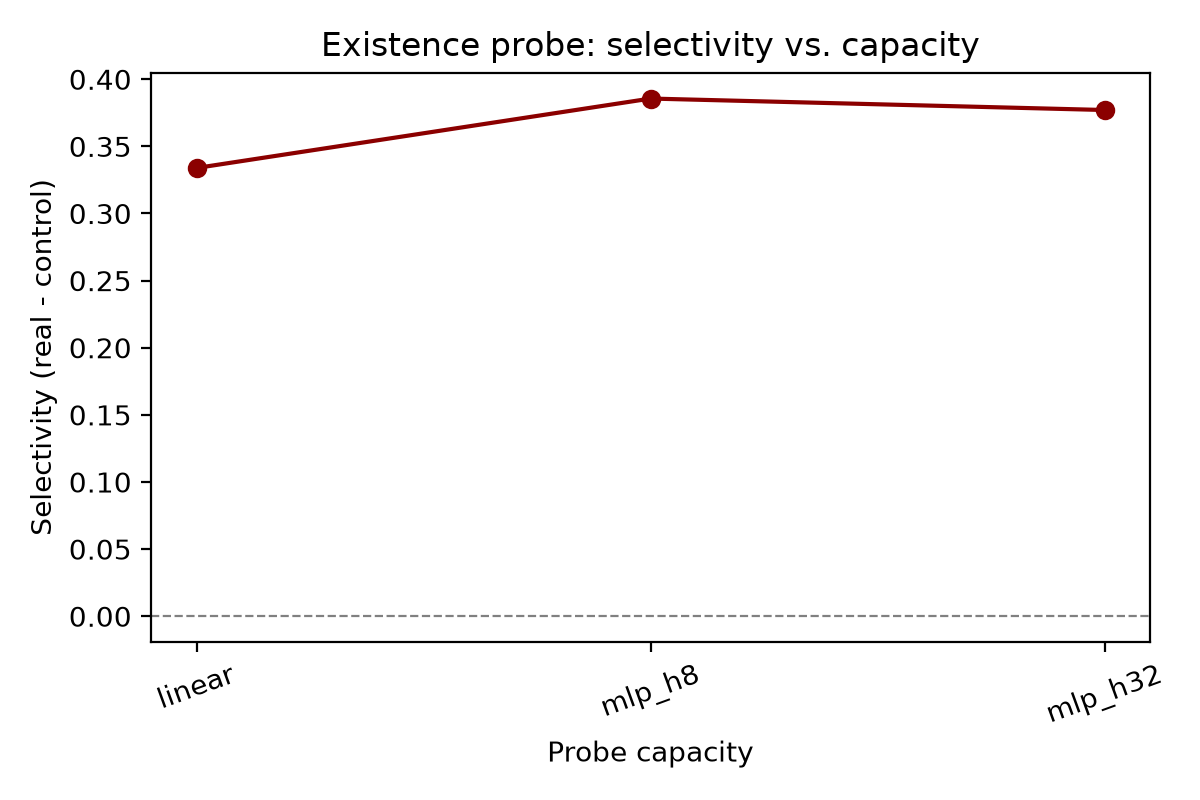
\includegraphics[width=\textwidth]{results/figures/capacity_selectivity_existence.png}
\caption{Dependency existence.}
\end{subfigure}
\hfill
\begin{subfigure}[b]{0.48\textwidth}
\centering
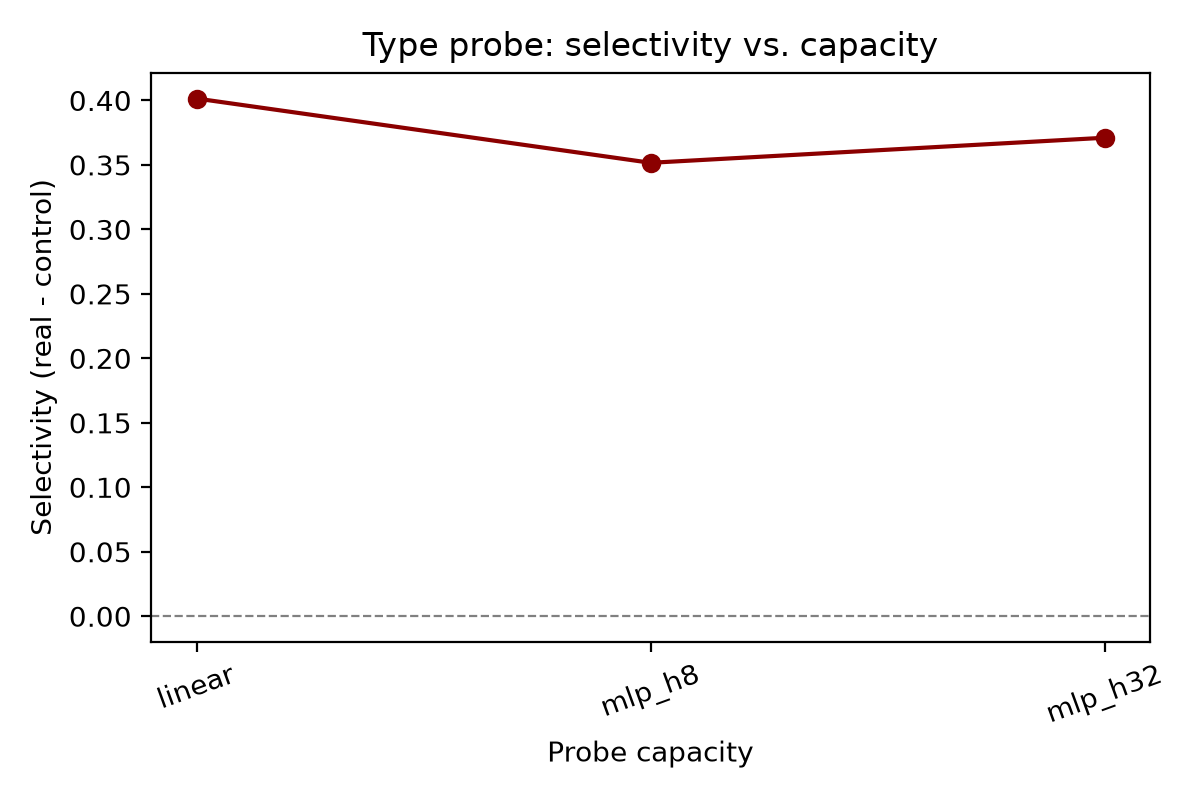
\includegraphics[width=\textwidth]{results/figures/capacity_selectivity_type.png}
\caption{Dependency type.}
\end{subfigure}

\caption{Selectivity as a function of probe capacity. Higher raw probe capacity does not produce a monotonic increase in selectivity.}
\label{fig:capacity-selectivity}
\end{figure}

\subsection{Experiment 3: Layer-Wise Selectivity}

The third experiment evaluates the 12 BERT attention layers separately. Each layer contributes 12 attention-head dimensions, allowing the same linear probing procedure to be applied to a substantially smaller but structurally coherent representation. A random subset of 12 dimensions from the full 144-dimensional representation serves as a dimensionality-matched baseline.

For dependency existence, the highest real-task accuracy occurs at layer 3, with an accuracy of 0.7699. Its control accuracy, however, is also relatively high at 0.5523, resulting in a selectivity of only 0.2176. In contrast, layer 7 achieves a slightly lower real-task accuracy of 0.7687 but a much lower control-task accuracy of 0.4587, producing the highest layer-wise selectivity of 0.3100. Layers 5 and 6 also form a strong region, with selectivities of 0.2943 and 0.2997 respectively. The result therefore separates the layer with the highest raw accuracy from the layer with the strongest selective evidence.

For dependency-type prediction, the pattern is more concentrated. Layer 7 achieves both the highest real-task accuracy, 0.4404, and the highest selectivity, 0.2642. The next-highest selectivities are considerably lower: 0.1744 at layer 8 and 0.1734 at layer 6. Selectivity decreases substantially toward the final layers, reaching 0.0842 at layer 10 and 0.0686 at layer 11.

\begin{table}[htbp]
\centering
\small
\caption{Selected layer-wise results, including the highest-accuracy or highest-selectivity layers and the random 12-dimensional baseline.}
\label{tab:layer-results}
\begin{tabular}{llccc}
\toprule
\textbf{Task} & \textbf{Representation} & \textbf{Real Acc.} & \textbf{Control Acc.} & \textbf{Selectivity} \\
\midrule
Existence & Full 144-dim. & 0.8404 & 0.5065 & 0.3339 \\
Existence & Layer 3 & \textbf{0.7699} & 0.5523 & 0.2176 \\
Existence & Layer 7 & 0.7687 & 0.4587 & \textbf{0.3100} \\
Existence & Random 12-dim. & 0.7063 & 0.4789 & 0.2274 \\
\midrule
Type & Full 144-dim. & 0.7130 & 0.3116 & 0.4014 \\
Type & Layer 7 & \textbf{0.4404} & 0.1762 & \textbf{0.2642} \\
Type & Random 12-dim. & 0.2745 & 0.1596 & 0.1149 \\
\bottomrule
\end{tabular}
\end{table}

The random 12-dimensional baseline reaches a selectivity of 0.2274 for dependency existence and 0.1149 for dependency type. Several coherent layers outperform these baselines, but not every layer does so. For example, layer 3 has the highest existence accuracy among individual layers but its selectivity is slightly below the random-dimensional baseline. This provides another example of why raw accuracy and selectivity should not be treated as equivalent measures.

The complete layer-wise patterns are shown in Figure~\ref{fig:layerwise-selectivity}. For existence, selectivity rises through the middle layers and reaches its maximum at layer 7 before declining toward the upper layers. The type task shows an even sharper peak at layer 7.

\begin{figure}[htbp]
\centering

\begin{subfigure}[b]{0.48\textwidth}
\centering
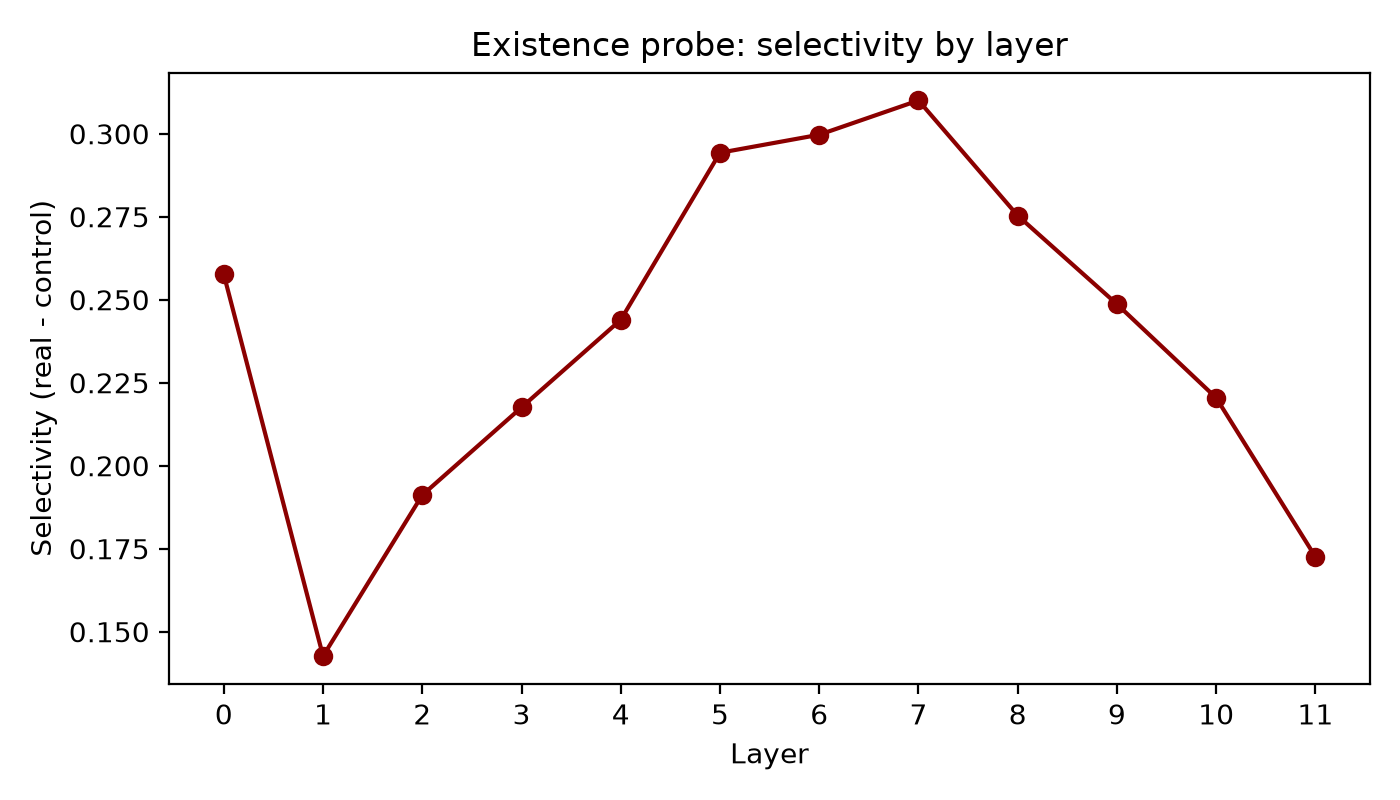
\includegraphics[width=\textwidth]{results/figures/layerwise_selectivity_existence.png}
\caption{Dependency existence.}
\end{subfigure}
\hfill
\begin{subfigure}[b]{0.48\textwidth}
\centering
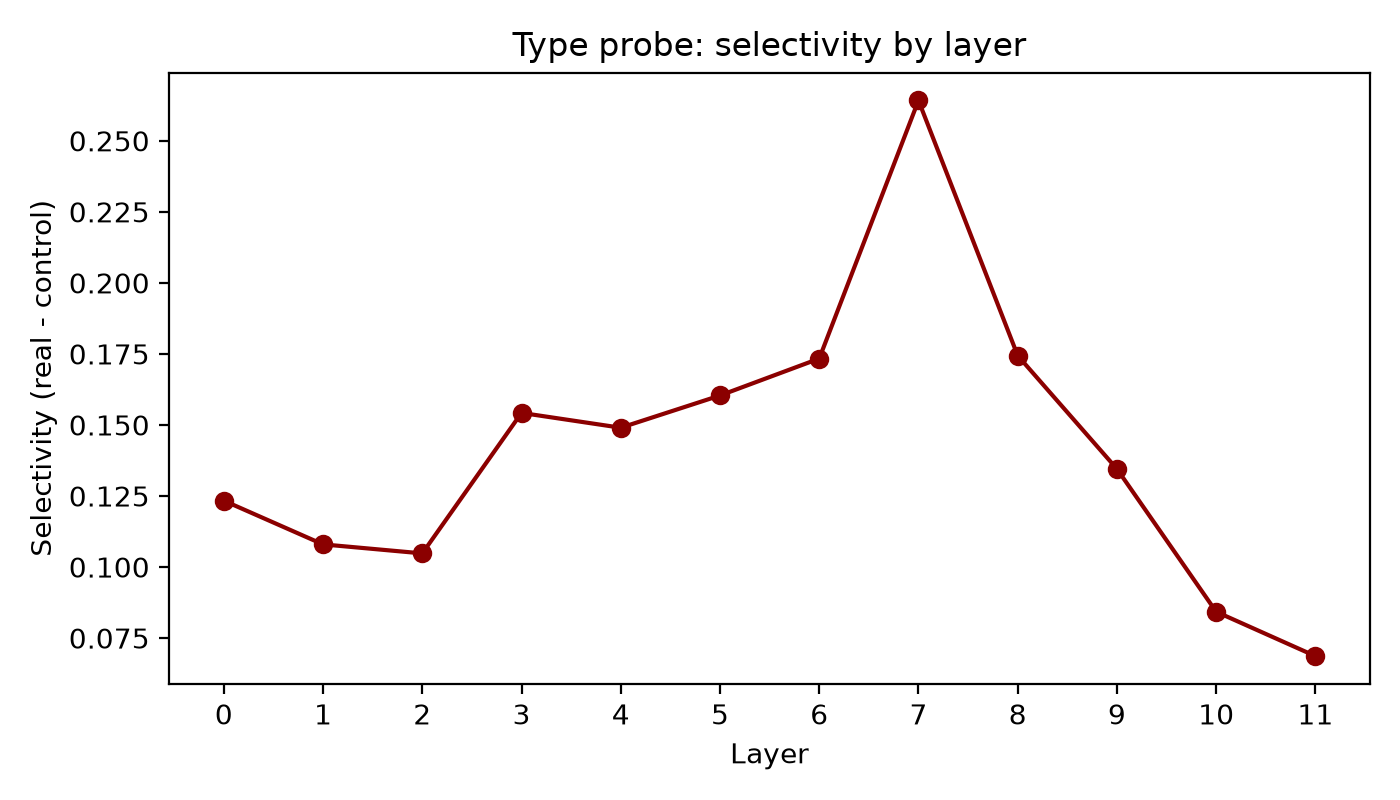
\includegraphics[width=\textwidth]{results/figures/layerwise_selectivity_type.png}
\caption{Dependency type.}
\end{subfigure}

\caption{Selectivity across BERT attention layers. Layer numbering follows the implementation and ranges from 0 to 11.}
\label{fig:layerwise-selectivity}
\end{figure}

Finally, no individual layer matches the complete 144-dimensional representation. The best single-layer existence accuracy is 0.7699 compared with 0.8404 for the full representation, while dependency-type accuracy reaches 0.4404 at its best single layer compared with 0.7130 using all attention heads. The same pattern appears in selectivity: the strongest individual layers reach 0.3100 and 0.2642 for existence and type, respectively, compared with 0.3339 and 0.4014 for the complete representation. The results indicate that syntactic information is not confined to a single attention layer, although particular middle layers, most notably layer 7, provide substantially more selective signals than others.

% ==================================================

% 5. DISCUSSION

% ==================================================

\section{Discussion}

The presented results demonstrate that syntactic dependency information is recoverable from BERT attention, but the interpretation of raw probe accuracy is not sufficient for evaluating probing results. For both probe capacity and layer depth, the configuration with the best linguistic task accuracy is not always the one with the best selectivity, which means that the control task performance should also be considered when analyzing probing results.

\subsection{Probe Accuracy versus Selectivity}

The probe-capacity experiment reveals that accuracy and selectivity are not equivalent measures. Even in the case of dependency existence,
while the MLP-32 achieves the highest real-task accuracy (0.8995) compared to the linear probe (0.8404), the highest selectivity (0.3856) is obtained by the MLP-8. The MLP-32 not only improves linguistic task accuracy but also performs better on the control task, thus, reducing the accuracy difference between the real and arbitrary labels.

The difference is more notable in the case of the dependency-type prediction: the MLP-32 achieves the highest real-task accuracy (0.7743) but the linear probe obtains the highest selectivity (0.4014). It supports the idea behind the control tasks proposed by Hewitt and Liang: if the same probe can also learn to make arbitrary associations with the given data, then the fact that it achieves high accuracy on the real task is a weaker indicator of the quality of the representation \cite{hewitt2019designing}.

This finding does not imply that the use of expressive probes is inherently wrong: the MLP-32 still has positive selectivity for both tasks, but the increase in the raw accuracy should be evaluated in terms of the control task performance.

\subsection{Distribution of Syntactic Information across Layers}

A similar observation can be made in the layer-wise results. In the case of dependency existence, layer~3 has the highest single-layer accuracy (0.7699) but the lowest selectivity (0.2176). At the same time, layer~7 has almost the same accuracy (0.7687) but the highest selectivity (0.3100). The layer from which syntax is easiest to predict is therefore not the most selective one.

In the case of the dependency-type prediction, layer~7 has the best results in terms of both accuracy (0.4404) and selectivity (0.2642). The performance of middle layers tends to be better than that of the later layers, which is in line with the previous findings about syntactic information being prominent in intermediate BERT layers \cite{tenney2019bert}. This also complements the observation by Clark et al.\ that particular attention heads are responsible for particular syntactic relations \cite{clark2019what}.

However, the results do not suggest that syntax is localized in a single layer. The best single-layer accuracy for the existence is 0.7699, while using the full 144-dimensional representation yields 0.8404. In the case of the type, the best layer reaches 0.4404, compared to 0.7130 for the full layer. This implies that syntax is distributed across several layers rather than being localized.

The random 12-dimensional baseline confirms this hypothesis: several coherent layers (particularly in the middle of the network) outperform the random subset, but this is not the case for every layer. Layer~3, for instance, has the best performance in terms of single-layer existence accuracy but its selectivity is still slightly lower than that of the random baseline. Layer~7 should therefore be considered the best layer in this experiment rather than the universal syntax layer in BERT, which also aligns with the recent findings about the limitation of mapping linguistic functions to depths in BERT \cite{niu2022pipeline}.

\subsection{Strengths and Limitations}

An advantage of the current study is that the real and control probes differ only in the target labels, using the same BERT attention features. Selectivity is also evaluated from two different angles: the probe capacity and the layer depth. Another strength is that the experiments cover both the dependency-existence and the dependency-type tasks, showing that the results are applicable to both classification problems.

The study has several limitations, however. First, only \texttt{bert-base-uncased} and the English Web Treebank are used. While this is a reasonable starting point, it does not allow making general claims about other models, languages, or datasets. Second, only attention weights are investigated: it is possible that the hidden state representations encode syntax in a different way. Third, the probe capacity is limited to one linear classifier, two MLPs, and the random 12-dimensional baseline.

Finally, while control tasks demonstrate how the performance of a probe changes depending on whether it is trained to recognize arbitrary labels, they do not make any claims about whether BERT actually uses the recovered syntactic information when making predictions. As previous work has shown, information being decodable from the representation does not necessarily imply that the model uses it \cite{rogers2020primer,belinkov2022probing}.

Overall, these results enable a more nuanced discussion of syntactic probing. Dependency information is indeed recoverable from BERT attention, but there is not enough evidence to claim that a model ``knows'' a linguistic property just because it can classify it with a high degree of accuracy. Both the choice of the probe and the layer affect the results, which is why selectivity should also be taken into consideration alongside raw accuracy.
% ==================================================

% 6.. Future WORK

% ==================================================

\section{Conclusion and Future Work}

This paper aimed to determine whether syntactic dependency information can be recovered from BERT attention, by evaluating probing performance against control tasks. Dependency-existence and type probing using \texttt{bert-base-uncased} demonstrated positive selectivity, showing that syntactic information is recoverable from attention. However, probe capacity did not consistently correlate with selectivity: while the MLP-32 achieved the highest raw accuracy on both tasks, the MLP-8 and linear probe yielded the highest selectivity for dependency existence and type, respectively.

The layer-wise analysis confirmed this result. While layer 3 achieved the highest single-layer accuracy on dependency existence, layer 7 achieved the highest selectivity. On the type task, layer 7 was also strongest on both metrics. These results are consistent with prior work finding syntactic information to be prominent in BERT's intermediate layers \cite{tenney2019bert}. Yet, no single layer demonstrated performance as strong as the full 144-dimensional attention vector, suggesting that syntactic information is not localized to a single layer.

The results of this paper demonstrate that control-task selectivity is an important metric that complements raw probing accuracy, and that high performance on a probing task should not be interpreted as evidence that a model ``understands'' a particular linguistic phenomenon.

Future work should compare pretrained BERT to an identically-structured randomly-initialized model to evaluate the contribution of pretraining to the observed results. This analysis could be extended to other Transformer-based models, as well as to other languages and treebank annotations. Additionally, the random 12-dimensional baseline could be repeated on multiple independently-sampled subsets to provide a stronger comparison and test the generalizability of these results.

% ==================================================
% REFERENCES
% ==================================================

\newpage

\addcontentsline{toc}{section}{References}

\bibliographystyle{plainnat}
\bibliography{references}

% ==================================================
% APPENDIX
% ==================================================

\newpage

% Trier requires Roman page numbering for the appendix
\pagenumbering{roman}
\setcounter{page}{1}

\appendix

\section{Supplementary Accuracy Figures}

The main text focuses on selectivity because it is the central measure used to evaluate the relationship between linguistic-task performance and control-task performance. For completeness, this appendix presents the corresponding real-task and control-task accuracy plots generated from the same experimental results.

\begin{figure}[htbp]
\centering

\begin{subfigure}[b]{0.48\textwidth}
\centering
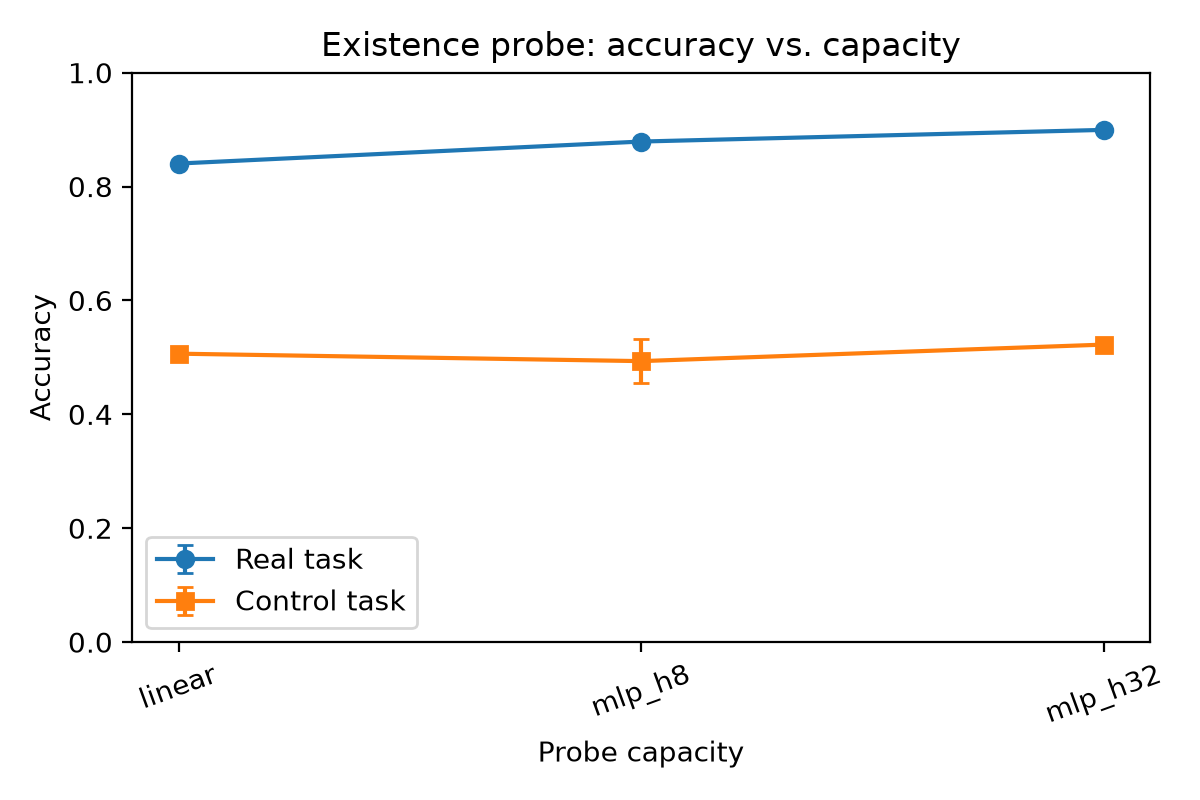
\includegraphics[width=\textwidth]{results/figures/capacity_sweep_existence.png}
\caption{Dependency-existence accuracy across probe capacities.}
\end{subfigure}
\hfill
\begin{subfigure}[b]{0.48\textwidth}
\centering
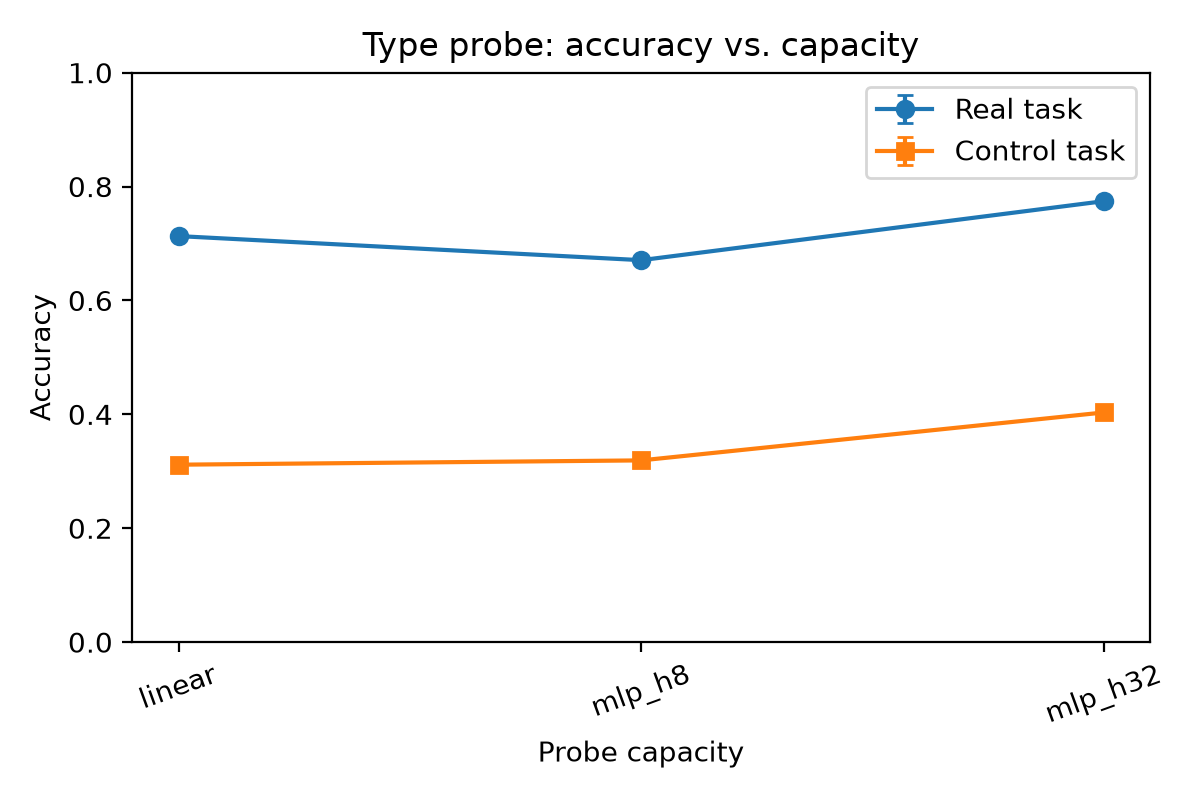
\includegraphics[width=\textwidth]{results/figures/capacity_sweep_type.png}
\caption{Dependency-type accuracy across probe capacities.}
\end{subfigure}

\caption{Real-task and control-task accuracy for the probe-capacity experiment. Error bars indicate the standard deviation across the configured runs.}
\label{fig:appendix-capacity-accuracy}
\end{figure}

\begin{figure}[htbp]
\centering

\begin{subfigure}[b]{0.48\textwidth}
\centering
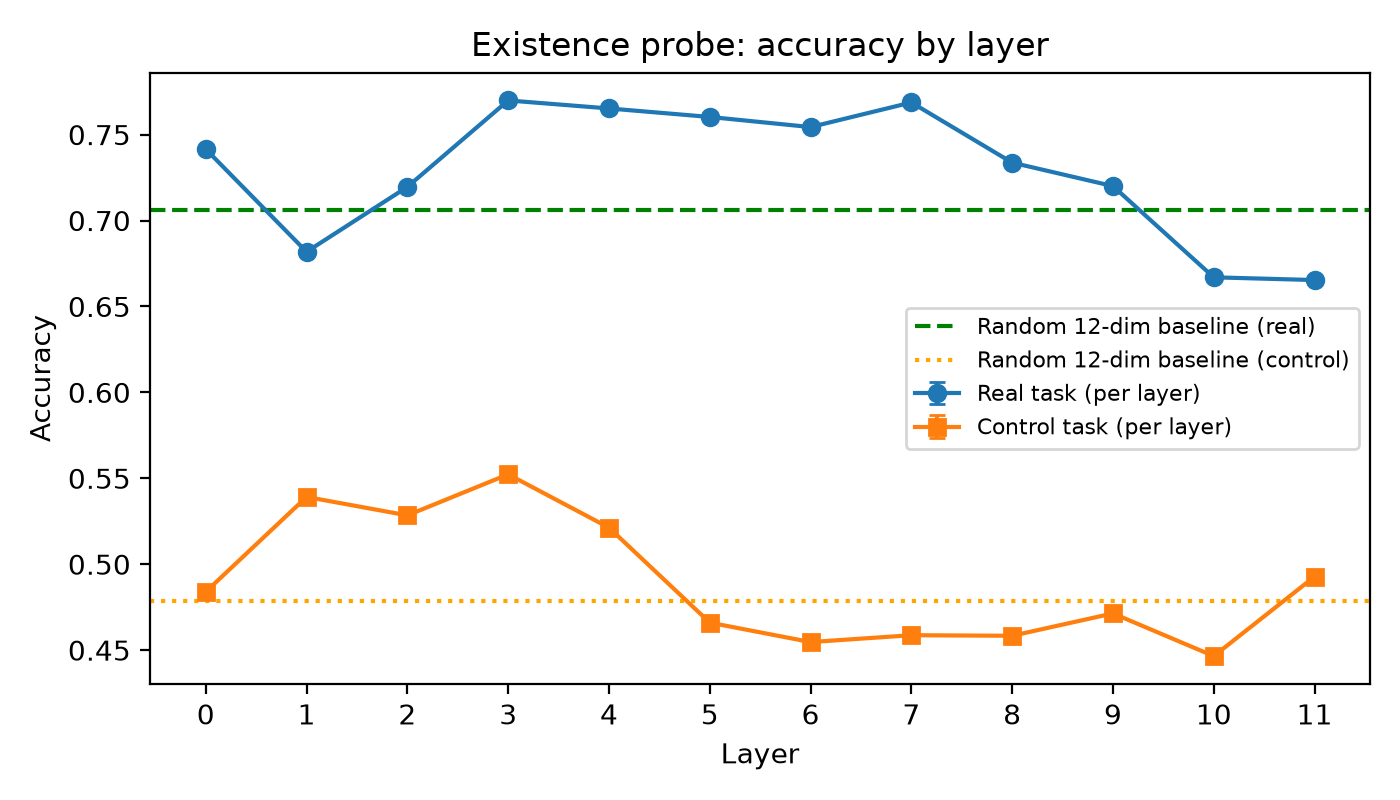
\includegraphics[width=\textwidth]{results/figures/layerwise_existence.png}
\caption{Dependency-existence accuracy by BERT layer.}
\end{subfigure}
\hfill
\begin{subfigure}[b]{0.48\textwidth}
\centering
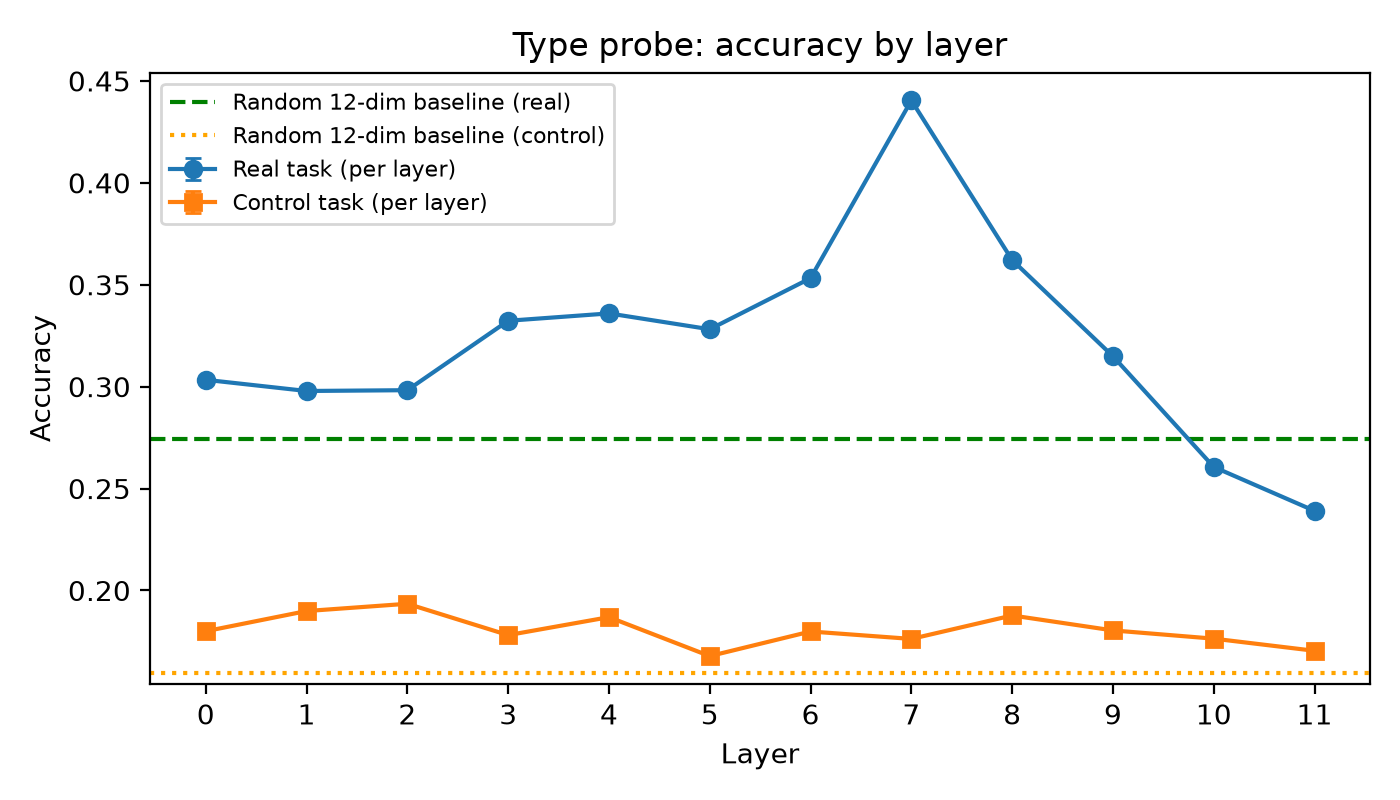
\includegraphics[width=\textwidth]{results/figures/layerwise_type.png}
\caption{Dependency-type accuracy by BERT layer.}
\end{subfigure}

\caption{Real-task and control-task accuracy for the layer-wise experiment. The horizontal reference lines show the corresponding random 12-dimensional baselines.}
\label{fig:appendix-layer-accuracy}
\end{figure}


\clearpage

\section{Complete Layer-Wise Results}

Tables~\ref{tab:appendix-existence-layers} and~\ref{tab:appendix-type-layers} report the complete numerical results for all 12 BERT attention layers and the random 12-dimensional baseline. The values correspond directly to the layer-wise result files used to generate the figures in Section~4.

\begin{table}[htbp]
\centering
\small
\caption{Complete layer-wise results for dependency existence.}
\label{tab:appendix-existence-layers}

\begin{tabular}{lccc}
\toprule
\textbf{Layer} & \textbf{Real Accuracy} & \textbf{Control Accuracy} & \textbf{Selectivity} \\
\midrule
0  & 0.7415 & 0.4839 & 0.2576 \\
1  & 0.6818 & 0.5391 & 0.1426 \\
2  & 0.7196 & 0.5284 & 0.1912 \\
3  & 0.7699 & 0.5523 & 0.2176 \\
4  & 0.7652 & 0.5213 & 0.2439 \\
5  & 0.7603 & 0.4660 & 0.2943 \\
6  & 0.7544 & 0.4547 & 0.2997 \\
7  & 0.7687 & 0.4587 & \textbf{0.3100} \\
8  & 0.7337 & 0.4583 & 0.2753 \\
9  & 0.7200 & 0.4713 & 0.2487 \\
10 & 0.6669 & 0.4465 & 0.2204 \\
11 & 0.6654 & 0.4928 & 0.1726 \\
\midrule
Random 12-dim. & 0.7063 & 0.4789 & 0.2274 \\
\bottomrule
\end{tabular}

\end{table}


\begin{table}[htbp]
\centering
\small
\caption{Complete layer-wise results for dependency-type prediction.}
\label{tab:appendix-type-layers}

\begin{tabular}{lccc}
\toprule
\textbf{Layer} & \textbf{Real Accuracy} & \textbf{Control Accuracy} & \textbf{Selectivity} \\
\midrule
0  & 0.3033 & 0.1800 & 0.1233 \\
1  & 0.2979 & 0.1899 & 0.1080 \\
2  & 0.2983 & 0.1935 & 0.1048 \\
3  & 0.3323 & 0.1781 & 0.1542 \\
4  & 0.3359 & 0.1869 & 0.1490 \\
5  & 0.3281 & 0.1678 & 0.1604 \\
6  & 0.3532 & 0.1799 & 0.1734 \\
7  & \textbf{0.4404} & 0.1762 & \textbf{0.2642} \\
8  & 0.3621 & 0.1877 & 0.1744 \\
9  & 0.3149 & 0.1804 & 0.1345 \\
10 & 0.2606 & 0.1763 & 0.0842 \\
11 & 0.2390 & 0.1704 & 0.0686 \\
\midrule
Random 12-dim. & 0.2745 & 0.1596 & 0.1149 \\
\bottomrule
\end{tabular}

\end{table}


\clearpage

\section{Reproducibility Resources}

The implementation used for the experiments, together with the generated result tables and figures, is available in the accompanying project repository:

\begin{center}
\url{https://github.com/vinsy2774/bert-attention-probe-selectivity}
\end{center}

The repository contains the scripts used for dependency-pair construction, control-task generation, BERT attention extraction, probe training, capacity analysis, layer-wise analysis, and figure generation. It also contains the CSV files from which the numerical results and plots reported in this paper were produced.

The experiments use the Universal Dependencies English Web Treebank, version r2.18, together with the pretrained \texttt{bert-base-uncased} model. Details of preprocessing, feature construction, probe architectures, control-task generation, and evaluation are provided in Section~3.

% ==================================================
% DECLARATION OF AUTHENTICITY
% ==================================================

\clearpage

\section*{Declaration of Authenticity}

I hereby declare that I have prepared this seminar paper independently and that I have used only the sources, materials, software, and tools indicated in the paper. All passages, ideas, or information taken directly or indirectly from published or unpublished sources have been identified and cited accordingly.

Generative AI tools were used only as supporting tools for language-related and editorial assistance, including paraphrasing, rephrasing, grammar correction, improving clarity, and organizing the structure of the paper. AI-generated suggestions were critically reviewed, revised, and verified by me before being included in the final version.

The underlying research topic, research question, experimental work, code execution, selection and presentation of results, and substantive scientific content are my own. The empirical results reported in this paper are based on the experiments and code described in the methodology and are not AI-generated. Generative AI was not used as a substitute for scientific sources, and all relevant academic claims were checked against the cited literature and the actual experimental results.

I take full responsibility for the accuracy, interpretation, and final content of this paper.

I further declare that this paper has not been submitted, in whole or in part, for assessment in another course or examination procedure.

\vspace{2.5cm}

\noindent
\begin{tabular}{p{6cm} p{6cm}}
\hrulefill & \hrulefill \\
Place and Date & Signature \\
\end{tabular}
\end{document}